% !TEX root = main.tex



- A breakdown of the embodied carbon emissions can be found in Figure  \ref{fig:embodied}... (brief discussion and design consideration)...

\begin{figure}[H]
\begin{center}
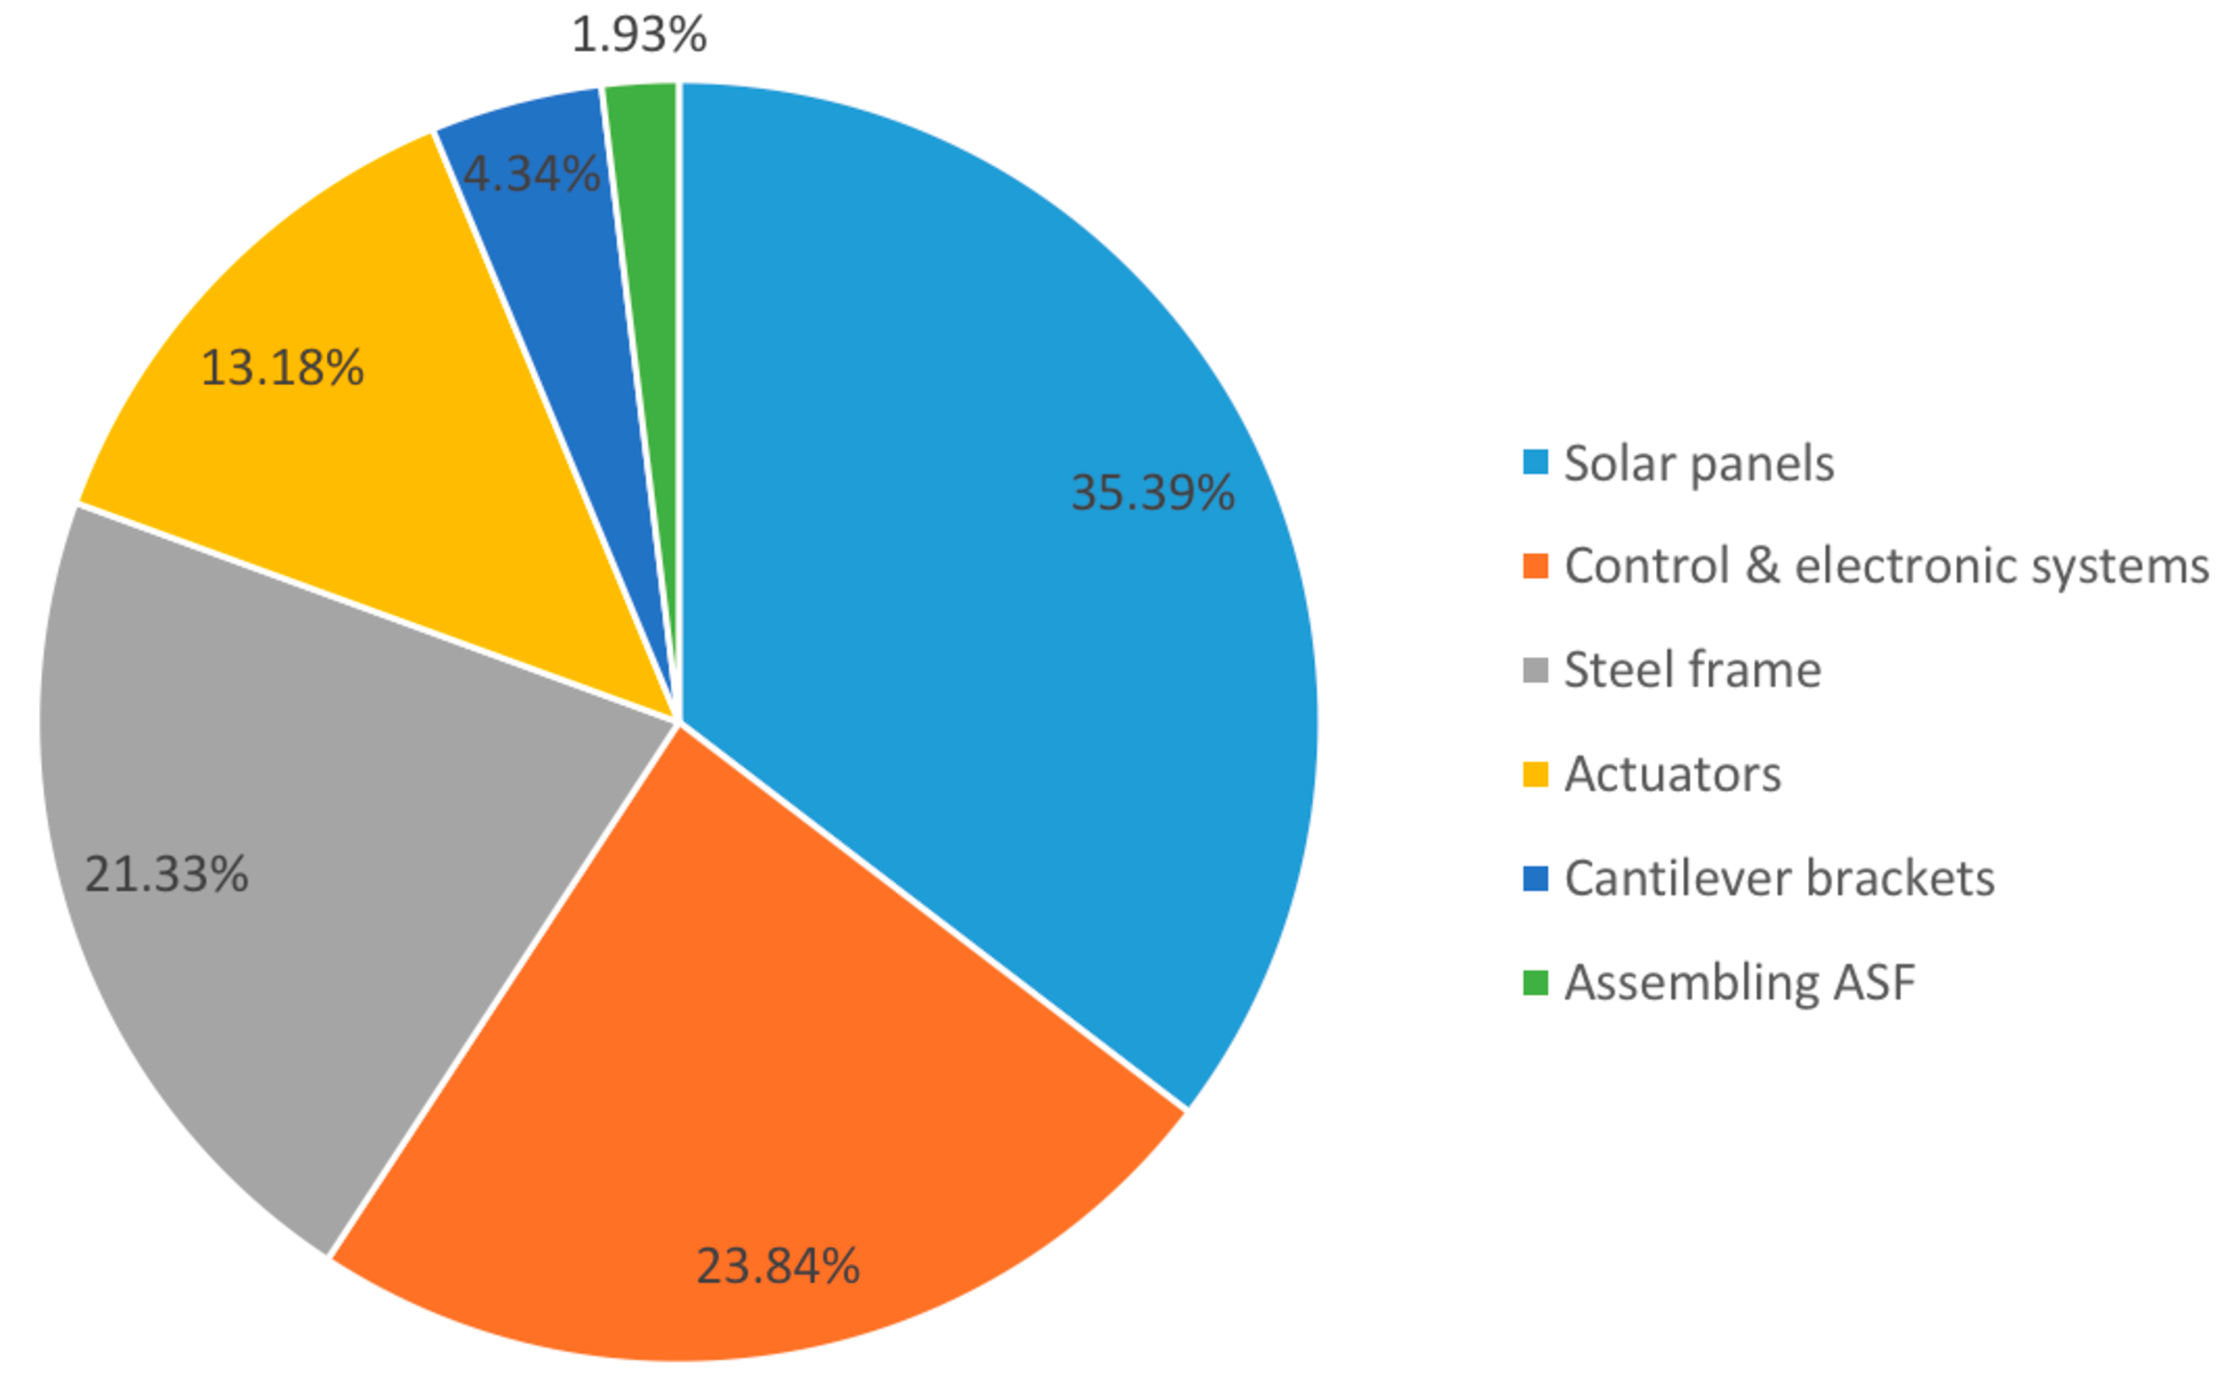
\includegraphics[width=10cm, trim= 0cm 0cm 0cm 0cm,clip]{pieembodied}
\caption{Breakdown of the embodied carbon emissions, it can be seen that xxxx has the greatest GWP contribution}
\label{fig:pembodied}
\end{center}
\end{figure}


\begin{figure}[H]
\begin{center}
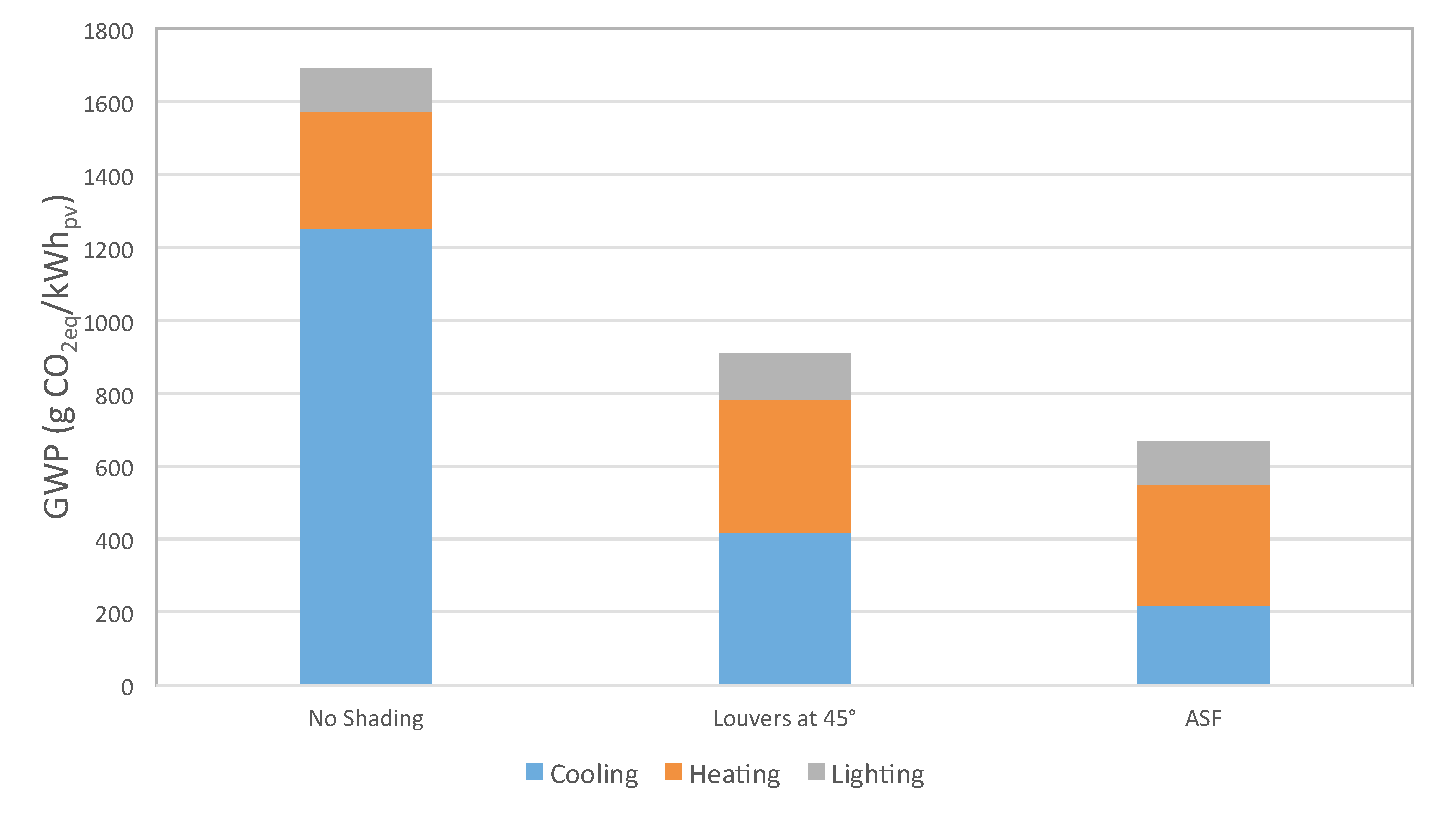
\includegraphics[width=10cm, trim= 0cm 0cm 0cm 0cm,clip]{buildingenergy}
\caption{Breakdown of the opperational carbon emissions, we can see a added savings of xxx compared to a static louvered shading system}
\label{fig:operational}
\end{center}
\end{figure}

- The results of the analysis can be summarized in Figure \ref{fig:waterfall}...

\begin{figure}[H]
\begin{center}
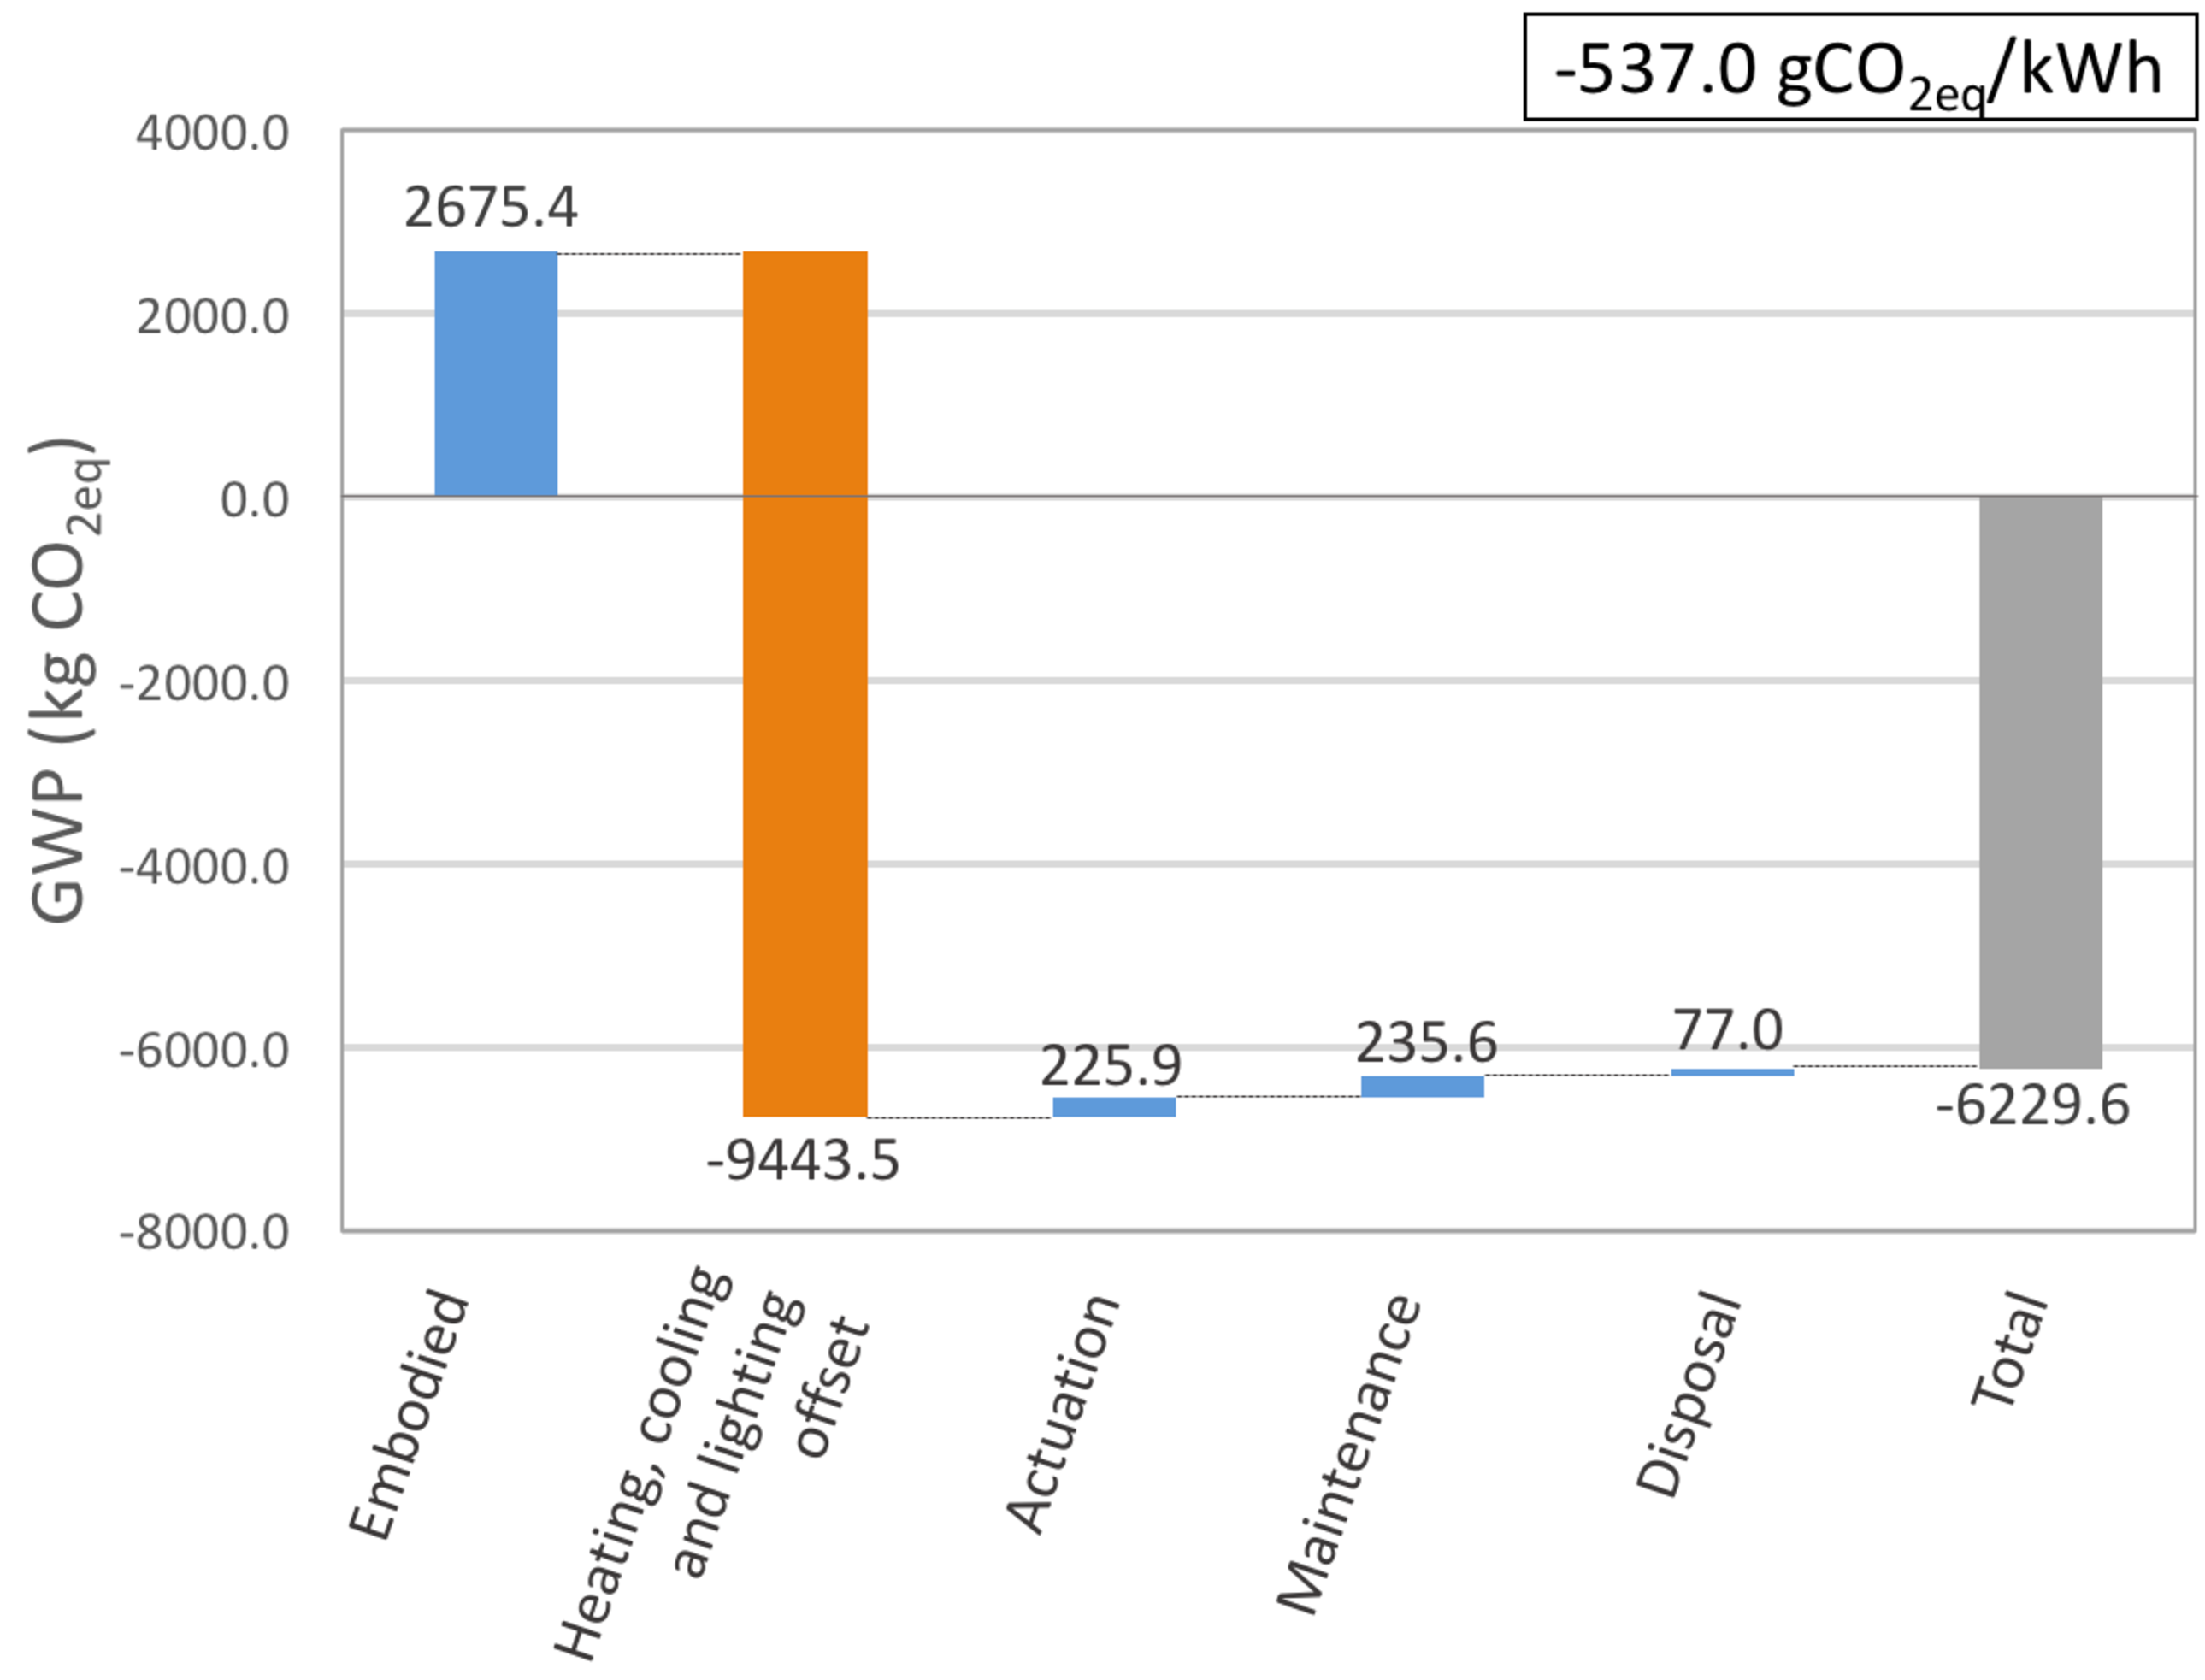
\includegraphics[width=10cm, trim= 0cm 0cm 0cm 0cm,clip]{waterfall}
\caption{Waterfall diagram of GWP of the ASF. The far left column details the embodied carbon emissions. The second bar details the emission reduction of the building through the smart shading algorithms of the ASF. The third column shows an increase of emissions through maintenance. The fourth column shows an increase in emissions in the disposal. This leaves us with a final emissions value. When we apply this value to Equation \ref{eq:solar} we obtain an emission factor per kwH of 173.8gCO2/kWh.}
\label{fig:waterfall}
\end{center}
\end{figure}


- As input parameters of production processes are stochastic, a Monte Carlo simulation is used to include this stochastic behavior in the results, as shown in Figure \ref{fig:monte}...

\begin{figure}[H]
\begin{center}

\includegraphics[width=10cm, trim= 0cm 0cm 0cm 0cm,clip]{monte}
\caption{Monte carlo simulation based on input uncertainties}
\label{fig:monte}
\end{center}
\end{figure}

% - Sourcing location greatly influences the embodied GWP. For photovoltaic panels, the majority of embodied emissions result from the use of electricity during production. The GWP per kwh of the Chinese electricity mix is 1145.8 ${\mathrm{gCO_2eq/kWh}}$, while in Switzerland this is only 119.6 ${\mathrm{gCO_2eq/kWh}}$.
% % cool - did we already discuss what other sensitivities to use?

% \begin{figure}[H]
% \begin{center}
% 
\includegraphics[width=10cm, trim= 0cm 0cm 0cm 0cm,clip]{sensitivity}
% \caption{Sensitivity analysis based on sourcing location}
% \label{fig:sensitivity}
% \end{center}
% \end{figure}
